\documentclass[12pt]{paper}

\usepackage{tikz}

\begin{document}
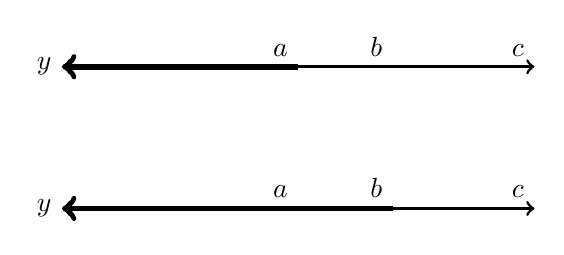
\begin{tikzpicture}[scale=0.6, line width = 1pt]

  \draw[<->] (0,3)--(10,3);
  \draw[<-, line width=.75mm](0,3)--(5,3);
  \node[left] at (0,3){$y$};
  \node[above left] at (5,3){$a$};
  \node[above left] at (7,3){$b$};
  \node[above left] at (10,3){$c$};

  
  \draw[<->] (0,0)--(10,0);
  \draw[<-,line width=.75mm](0,0)--(7,0);
  \node[left] at (0,0){$y$};
  \node[above left] at (5,0){$a$}; left
  \node[above left] at (7,0){$b$};
  \node[above left] at (10,0){$c$};

  
\end{tikzpicture}

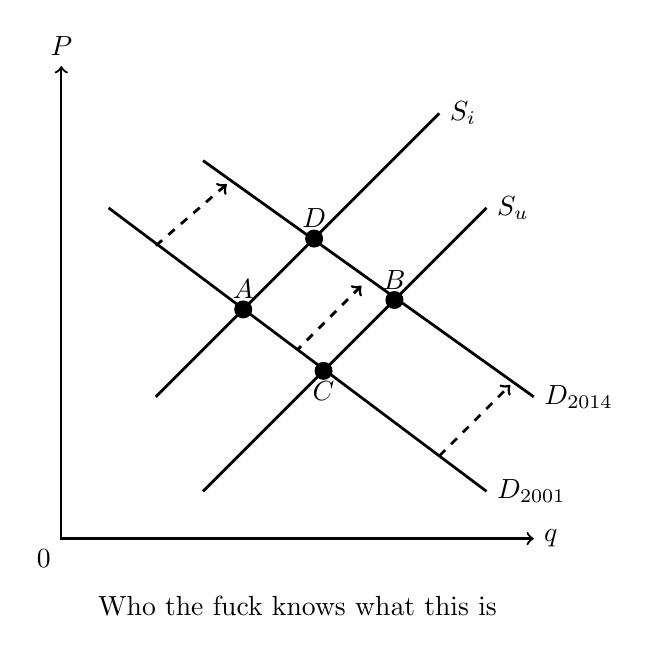
\begin{tikzpicture}[scale=0.6, line width = 1pt]

\draw[thick,<->] (0,10) node[above]{$P$}--(0,0)--(10,0) node[right]{$q$};

\node [below left] at (0,0) {$0$};

\draw (3,1)--(9,7);
\node [right] at (9,7){$S_u$};
\draw (2,3)--(8,9);
\node[right] at (8,9){$S_i$};

\draw [->,dashed] (8,1.75)--(9.5,3.25);
\draw [<-,dashed] (6.35,5.35)--(5,4);
\draw [->,dashed] (2,6.2)--(3.5,7.5);

\fill (3.85,4.85) circle (.075in);
\node[above] at (3.85,4.85){$A$};
\fill (7.05,5.05) circle (.075in);
\node[above] at (7.05,5.05){$B$};
\fill (5.55,3.55) circle (.075in);
\node[below] at (5.55,3.55){$C$};
\fill (5.35,6.35) circle (.075in);
\node[above] at (5.35,6.35){$D$};

\draw (1,7)--(9,1);
\node [right] at (9,1){$D_{2001}$};
\draw (3,8)--(10,3);
\node [right] at (10,3){$D_{2014}$};

\node [below] at (5,-1){Who the fuck knows what this is};

\end{tikzpicture}

\end{document}
